\documentclass{article}
\usepackage[utf8]{inputenc}
\usepackage{amsmath}
\usepackage{amsfonts}
\usepackage{graphicx}
\graphicspath{ {./images/} }

\title{Statistical inference}
\author{Gabriel Aguiar}
\date{October 2019}

\begin{document}

\maketitle

Claude Shannon, father of Information Theory, built in 1948 what became known as "Shannon's Entropy". Claude wanted to describe a "Surprise" function $S$ that varies according to the probability $p$ of a given event $x$. This function should tend to infinity when p tends to 0 and equals 0 when p is 1 (as in the following chart).

\hfill

\hfill

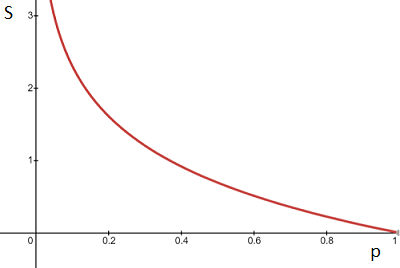
\includegraphics{graph}

\hfill

Thus, an event with zero probability would be very surprising, while a probability event of 1 would be quite expected.

Shannon came to call this function $S$ "Information," denoted by $h)$. That way, expressed:

\hfill

$h(x) = log_{2} \; \frac{1}{p(x)}$, with $0 \leq p \leq 1$

\hfill

The dimension of h is now called bit.

\hfill

\hfill

Shannon further defined the entity "entropy" associated with a state of possible events as:

\hfill

$S \equiv \sum\limits_{x} \; p(x) \; log_{2} \; \frac{1}{p(x)} = \sum\limits_{x} \; p(x) \; h(x)$

\hfill

$x \in A_{x}$ ($x$ alphabet)

\end{document}